\section{OpenStack Sahara}

\subsection{Introduction}
\begin{frame}
	\frametitle{The intersection of Hadoop and OpenStack}
	\begin{figure}
		
\includegraphics[width=0.2\linewidth]{images/hadoop-openstack.jpg}
	\end{figure}
	\begin{figure}
		
\includegraphics[width=0.4\linewidth]{images/sahara-logo-square.png}
	\end{figure}
\end{frame}


\begin{frame}
	\frametitle{Mission}
Sahara’s mission is to provide a scalable data processing stack and associated management interfaces. Sahara delivers on that mission by providing the ability to rapidly create and manage Apache Hadoop clusters and easily run workloads across them. All on OpenStack managed infrastructure, without having to deal with the details of cluster management.

With full cluster lifecycle management, provisioning, scaling and termination, Sahara allows the user to select different Hadoop versions, cluster topology and node hardware details.
\end{frame}

\begin{frame}
	\frametitle{Sahara key features and use cases}
	\begin{itemize}
		\item Fast and agile Hadoop cluster deployment
		\item An extensible framework for management and provisioning components
		\item Run Hadoop workloads in few clicks without expertise in Hadoop operations
		\item “Analytics as a Service” utilization of unused compute capacity for ad-hoc or bursty analytic workloads
		\item Sahara supports different types of jobs: MapReduce, Hive, Pig and Oozie workflows. The data could be taken from various sources: Swift, HDFS, NoSQL and SQL databases. It also  supports various provisioning plugins.
		\item The intersection of two of the largest open source movements
		\item OpenStack provides  the foundation and hub of innovation for cleanly managing infrastructure resources. While Apache Hadoop™ serves as the core and innovation driver for storing and processing data.
	\end{itemize}
\end{frame}

\begin{frame}
	\frametitle{Sahara Functionality}
	\begin{itemize}
		\item Bringing up cluster
		\item Configure it along the way
		\item Scale cluster
		\item Terminate cluster
		\item Job execution (Elastic Data Processing)
	\end{itemize}
\end{frame}

\begin{frame}
	\frametitle{OpenStack Layers}
	\begin{figure}
		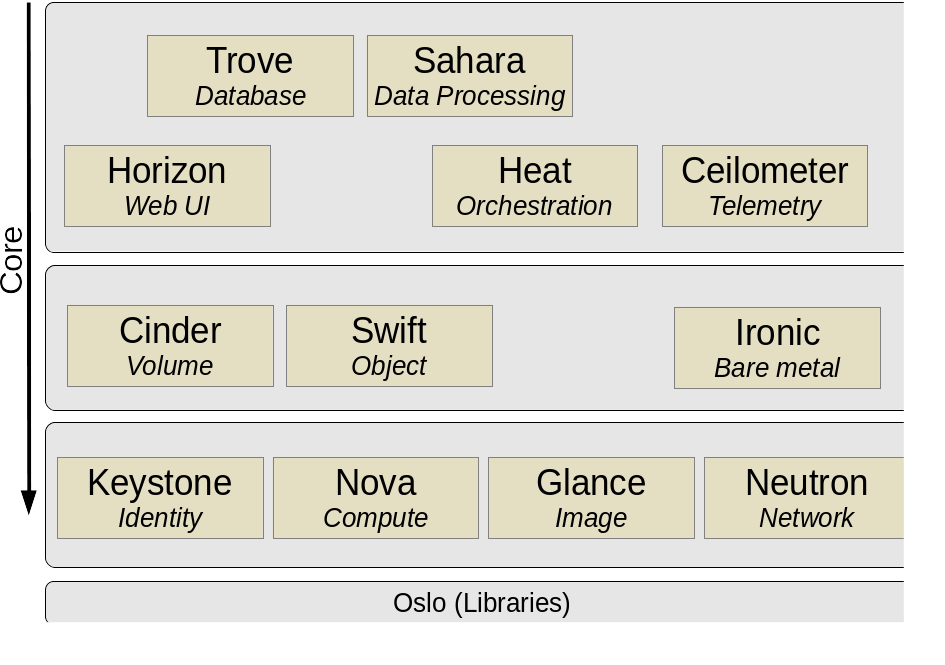
\includegraphics[width=1\linewidth]{images/openstack_layers.png}
	\end{figure}
\end{frame}

\begin{frame}
	\frametitle{Sahara Architecture}
	\begin{figure}
		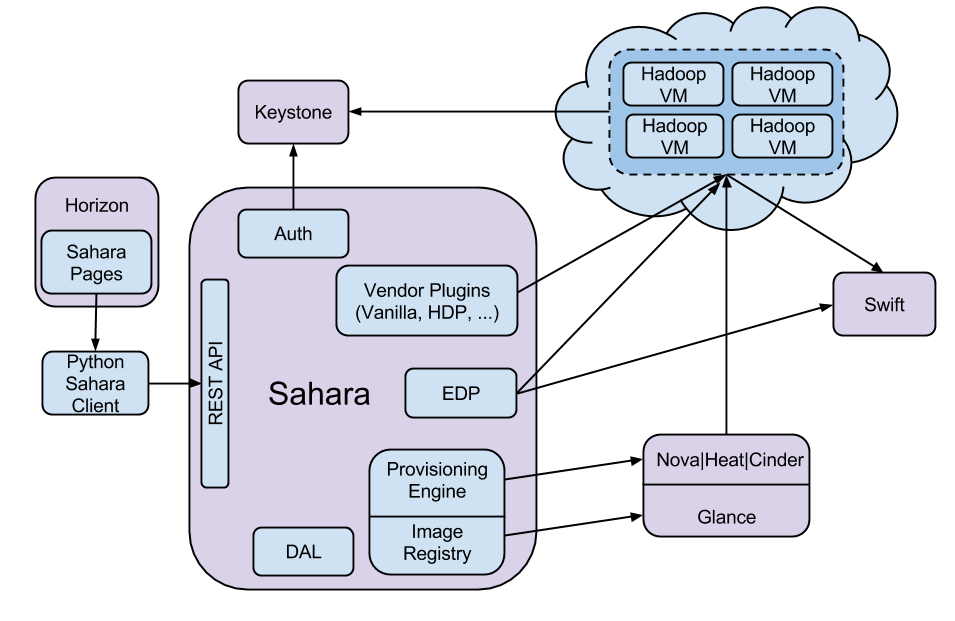
\includegraphics[width=1\linewidth]{images/sahara-architecture.png}
	\end{figure}
\end{frame}

\begin{frame}
	\frametitle{OpenStack Integration}
	\begin{figure}
		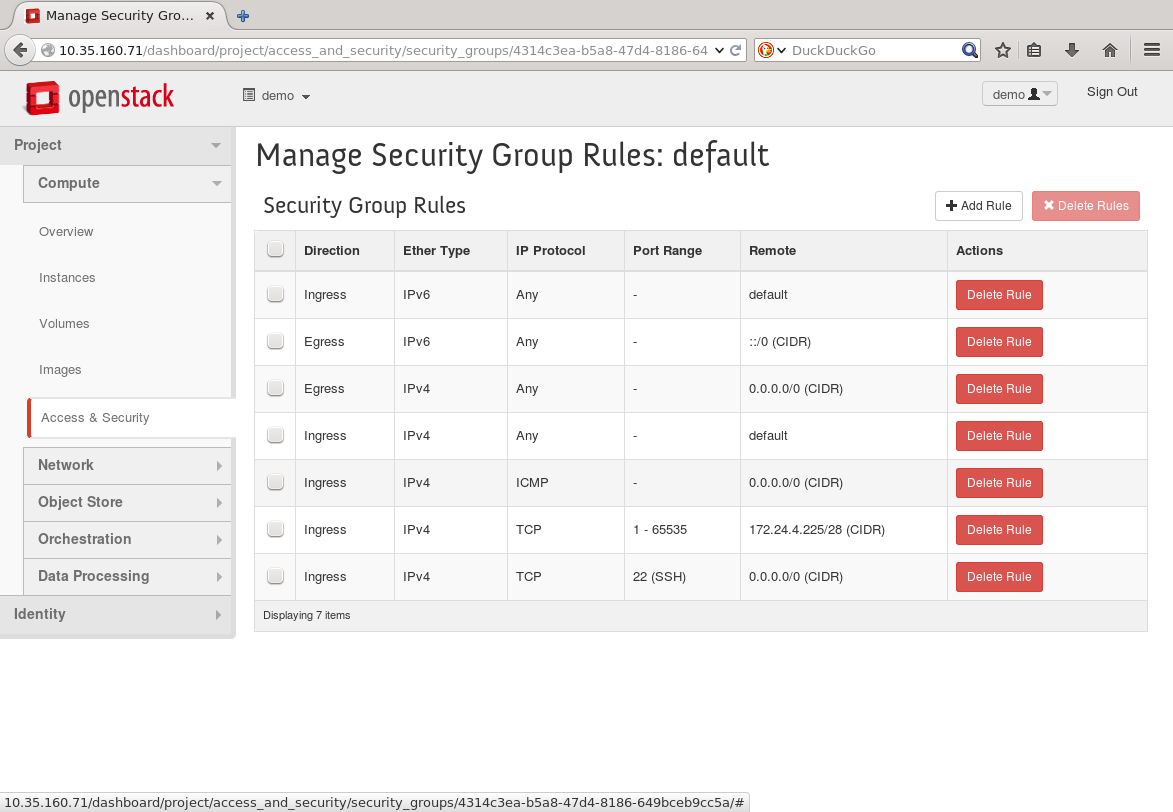
\includegraphics[width=1\linewidth]{images/sahara-securitygroup.png}
	\end{figure}
\end{frame}


\subsection{Slided demo}
\begin{frame}
	\frametitle{Upload Sahara image}
	\begin{figure}
		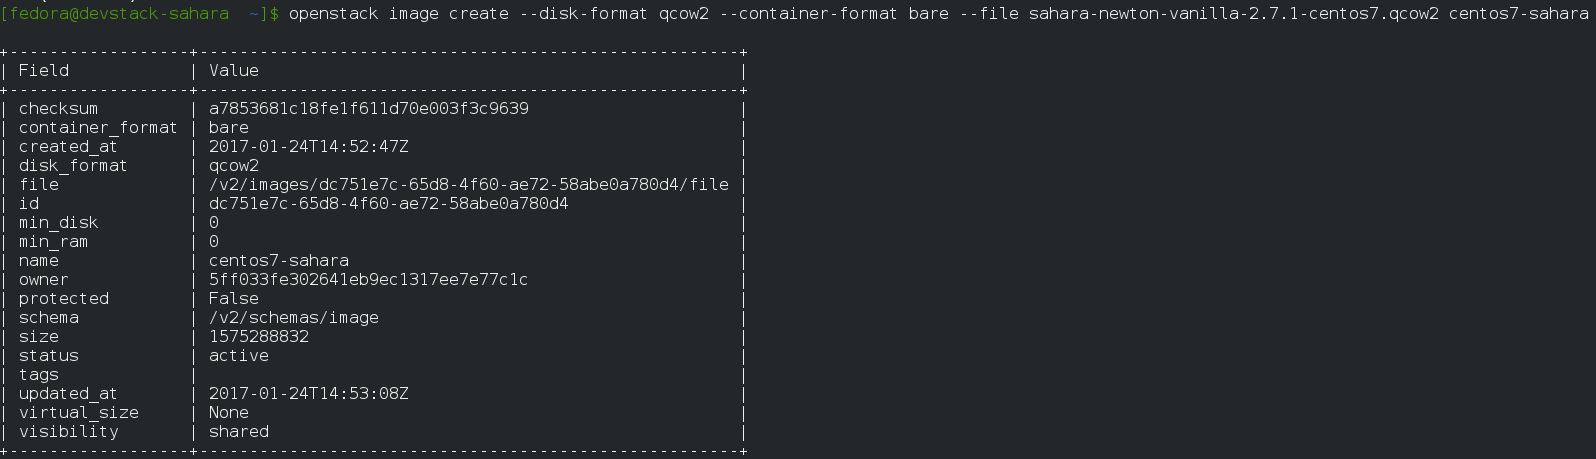
\includegraphics[width=1\linewidth]{images/1-upload_sahara_image.png}
	\end{figure}
\end{frame}

\begin{frame}
	\frametitle{Register Sahara image}
	\begin{figure}
		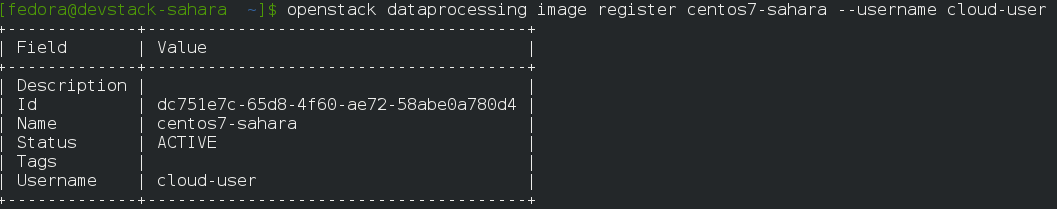
\includegraphics[width=1\linewidth]{images/2-register_sahara_image.png}
	\end{figure}
\end{frame}

\begin{frame}
	\frametitle{Configure Hadoop plugin}
	\begin{figure}
		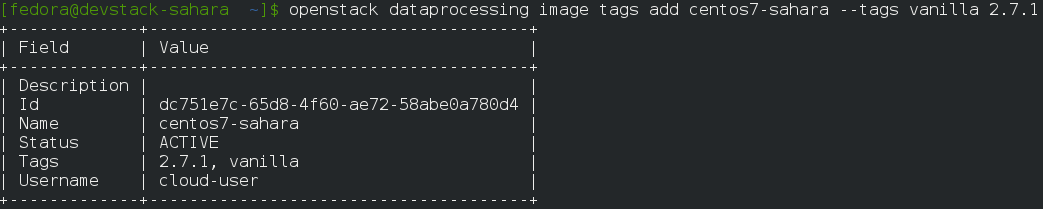
\includegraphics[width=1\linewidth]{images/3-configure_hadoop_plugin_tags.png}
	\end{figure}
\end{frame}

\begin{frame}
	\frametitle{Available Hadoop plugins}
	\begin{figure}
		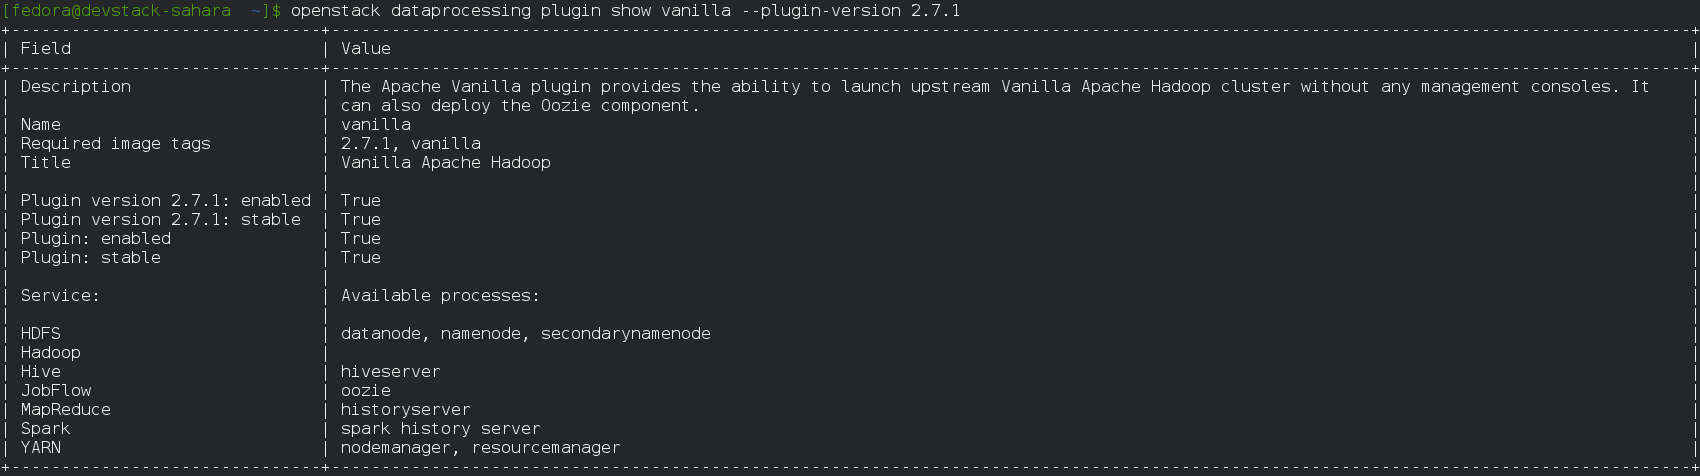
\includegraphics[width=1\linewidth]{images/4-available_sahara_plugins.png}
	\end{figure}
\end{frame}

\begin{frame}
	\frametitle{Create node templates}
	\begin{figure}
		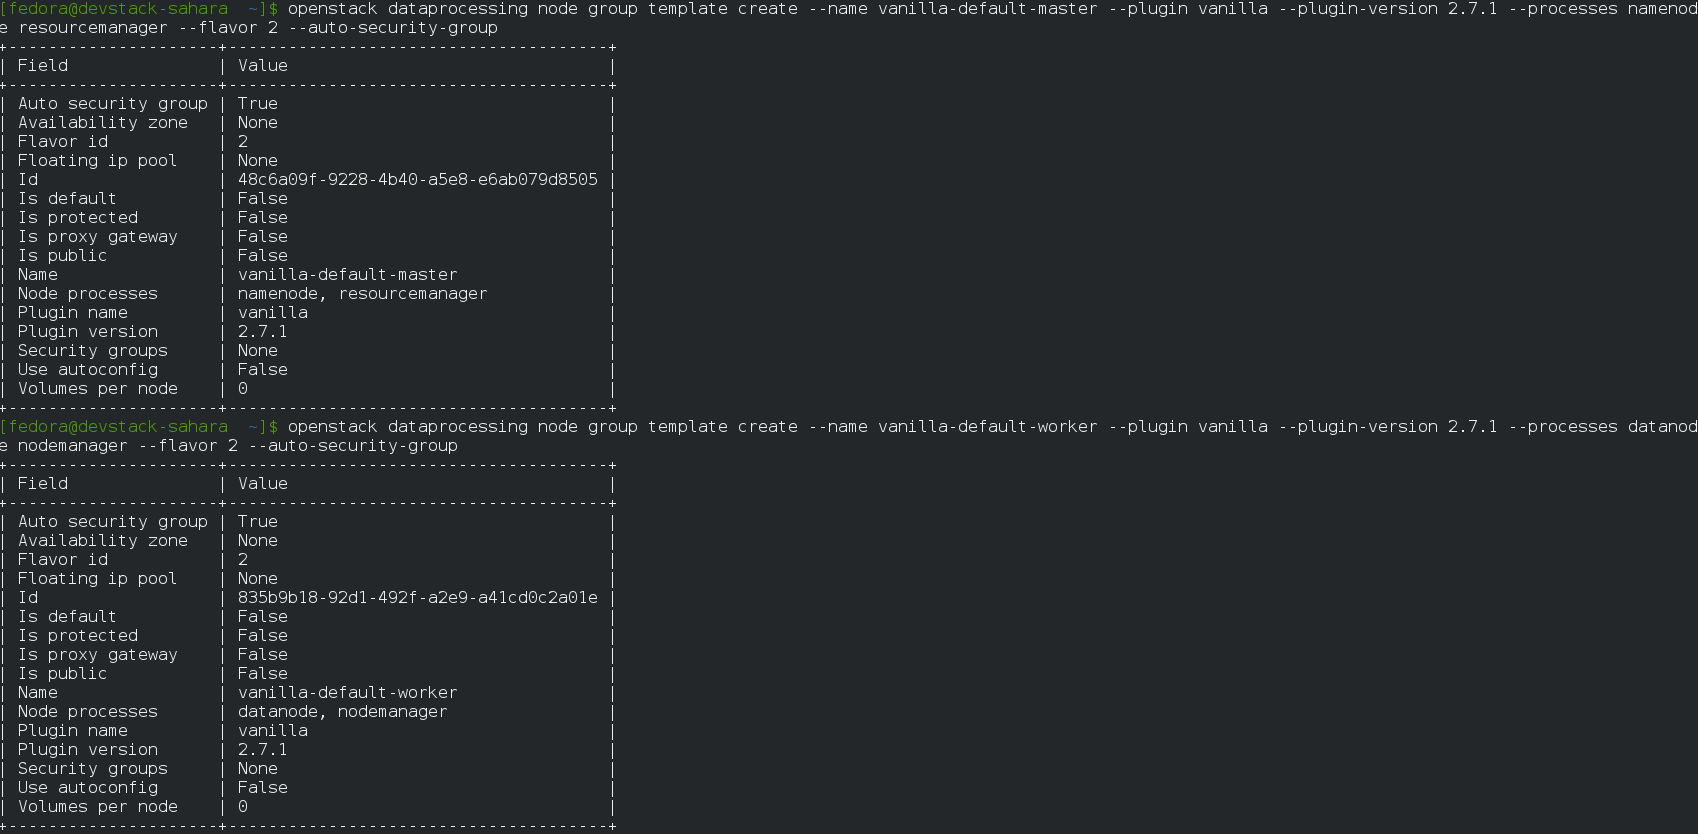
\includegraphics[width=1\linewidth]{images/5-create_node_templates.png}
	\end{figure}
\end{frame}

\begin{frame}
	\frametitle{Create cluster template}
	\begin{figure}
		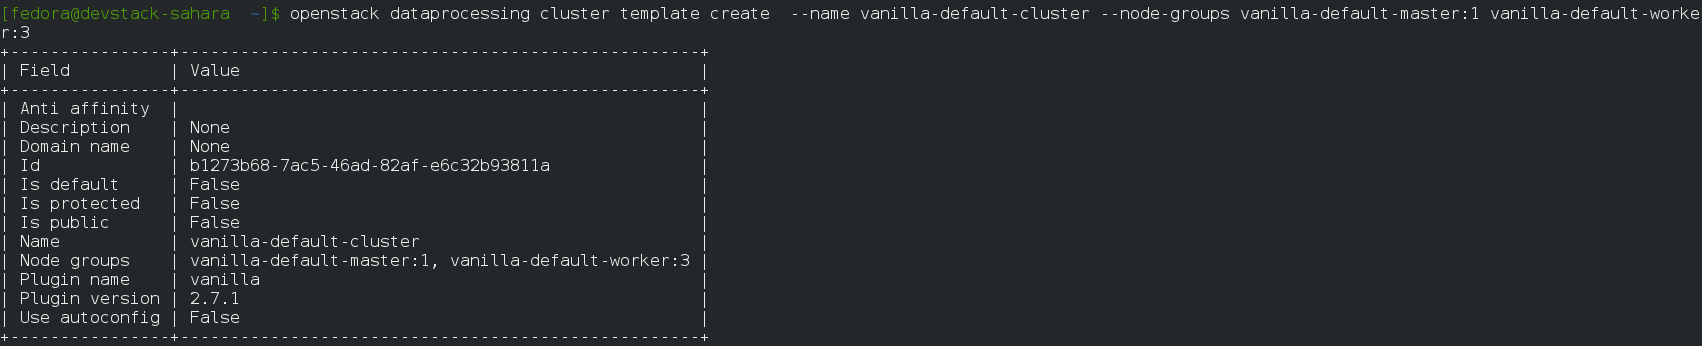
\includegraphics[width=1\linewidth]{images/6-create_cluster_template.png}
	\end{figure}
\end{frame}

\begin{frame}
	\frametitle{Create cluster}
	\begin{figure}
		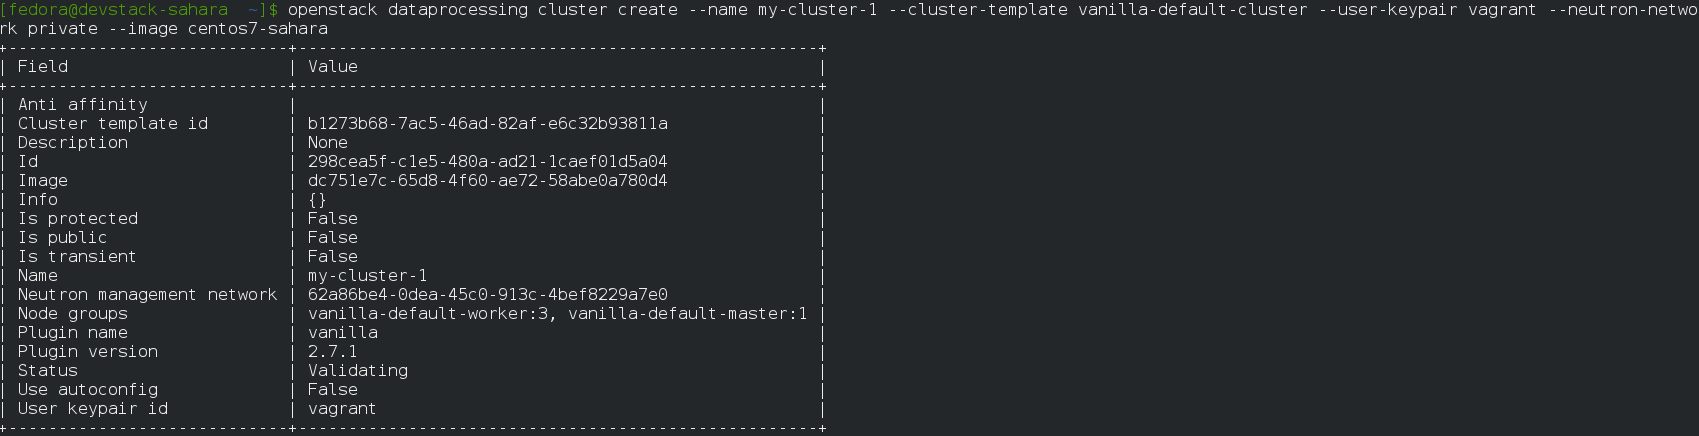
\includegraphics[width=1\linewidth]{images/7-create_cluster.png}
	\end{figure}
\end{frame}

\begin{frame}
	\frametitle{Show cluster}
	\begin{figure}
		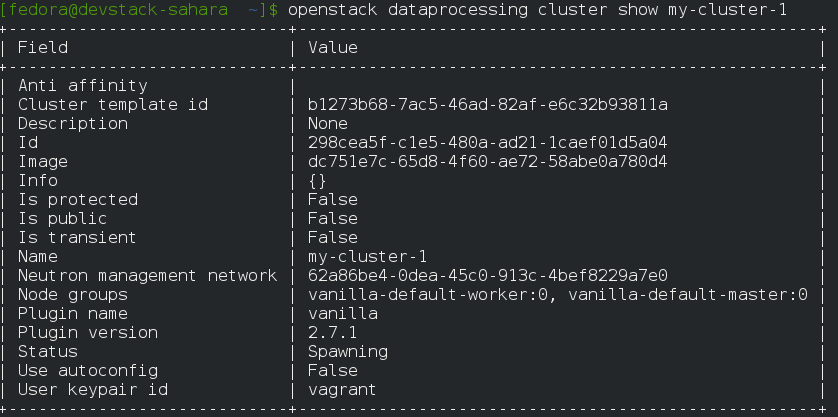
\includegraphics[width=1\linewidth]{images/8-show_cluster.png}
	\end{figure}
\end{frame}
